% =====================================================================
%  EPD-SDIA-4112 -- Statistique Bayesienne -- Master 1 SDIA
%  CHAPITRE 2 : Distributions a priori et a posteriori
%  Fichier C : sections 2.4 (robustesse, sensibilite, shrinkage) et 2.5 (synthese)
% =====================================================================

% ---------------------------------------------------------------- 1
% [suite]
\begin{frame}{2.4 — « Et si mon a priori est faux ? »}
% [rogna]
\small
\begin{kbox}[Trois questions, trois réponses]
\begin{enumerate}
  \item \textbf{À quelle vitesse} les données prennent-elles le dessus ?
        Réponse : l'information s'accumule en $1/\sqrt{n}$, le décalage du prior
        décroît en $1/n$.
  \item \textbf{Combien de poids} donner à un historique ? Réponse : le
        \emph{power prior}, un curseur $a_0 \in [0,1]$ à justifier.
  \item \textbf{Que faire de plusieurs groupes} quand certains sont petits ?
        Réponse : un prior hiérarchique, c'est-à-dire du \emph{shrinkage}.
\end{enumerate}
\end{kbox}
\vspace{1mm}
\end{frame}

% [suite]
\begin{frame}{2.4 — « Et si mon a priori est faux ? » (suite)}
\begin{columns}[t]
\begin{column}{0.55\textwidth}
\begin{ebox}[Le cadre : sensibilité]
On ne cherche plus « le bon prior » (il n'existe pas) mais \textbf{l'effet du choix
de prior}. Sur une proportion $p$ réellement égale à $0{,}35$, avec un
$\mathrm{Beta}(50,50)$ (centré sur $0{,}5$, donc \emph{faux}) :
\begin{center}
\begin{tabular}{@{}lcccc@{}}
\toprule
\textbf{Prior} & $n = 10$ & $n = 100$ & $n = 1000$ & $n = 3000$ \\
\midrule
Beta$(1,1)$   & 0,4167 & 0,3627 & 0,3303 & 0,3441 \\
Beta$(2,2)$   & 0,4286 & 0,3654 & 0,3307 & 0,3442 \\
Beta$(5,3)$   & 0,5000 & 0,3796 & 0,3323 & 0,3447 \\
Beta$(50,50)$ & 0,4909 & 0,4300 & 0,3455 & 0,3490 \\
\bottomrule
\end{tabular}
\end{center}
\hfill\footnotesize moyenne a posteriori ($p$ vrai $= 0{,}35$)
\end{ebox}
\end{column}
\begin{column}{0.42\textwidth}
\begin{wbox}[Lecture honnête du tableau]
À $n = 10$, le prior \emph{faux} déplace la réponse de $0{,}15$ (0,49 contre 0,35) :
la conclusion est pilotée par le prior. À $n = 3000$, tous les priors se recollent
autour de $0{,}34$–$0{,}35$ : \textbf{les données gagnent, mais lentement} et sans
jamais effacer complètement le décalage (voir frame suivante).
\end{wbox}
\end{column}
\end{columns}
\end{frame}

% ---------------------------------------------------------------- 2
% [rogna]
% [rogna]
\begin{frame}{La vitesse de dominance des données}
\begin{center}
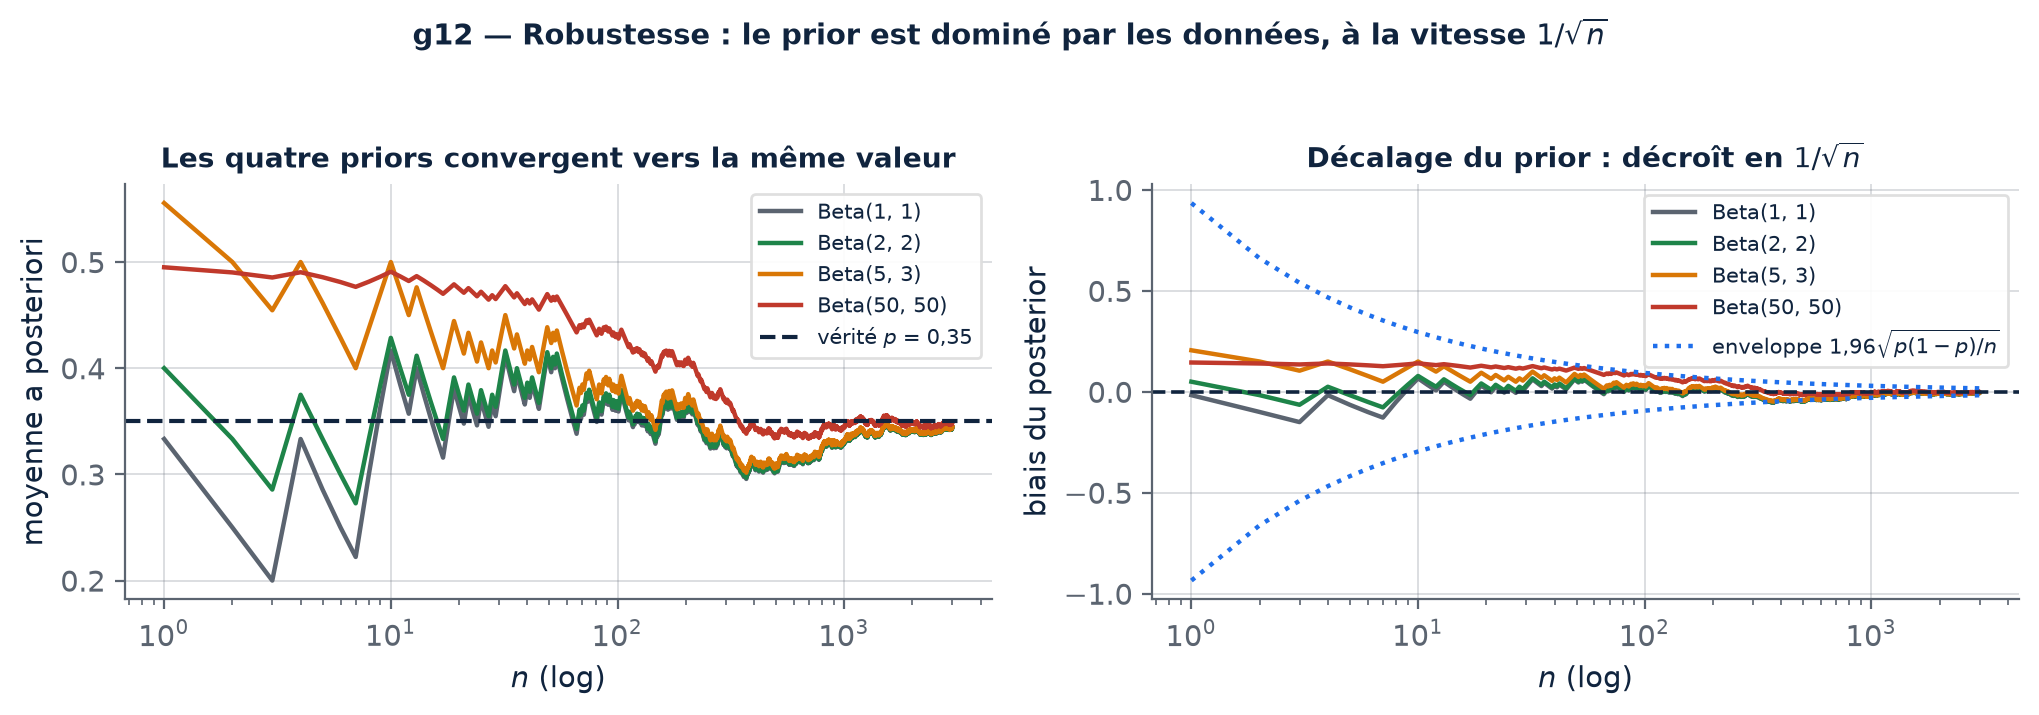
\includegraphics[width=0.72\textwidth]{g12_sensibilite_n.png}
\end{center}
\vspace{-1mm}
\begin{columns}[t]
\begin{column}{0.53\textwidth}
\begin{ebox}[Ce que mesurent les courbes]
L'écart-type de la loi des données vaut $\sqrt{p(1-p)/n}$ et suit exactement
la loi $1/\sqrt{n}$ : $0{,}1508$ pour $n = 10$, $0{,}0477$ pour $n = 100$,
$0{,}0151$ pour $n = 1000$, $0{,}0087$ pour $n = 3000$
(rapport $0{,}1508/0{,}0087 = 17{,}3 = \sqrt{300}$).
\end{ebox}
\end{column}
\begin{column}{0.44\textwidth}
\begin{kbox}[La bonne façon de le dire]
Le posterior se resserre comme $1/\sqrt{n}$, mais la \emph{position} de son centre
n'est pas garantie : c'est le décalage résiduel du prior, qui décroît seulement
en $1/n$ (frame suivante). Retenir la phrase : \textbf{la précision s'achète en
$1/\sqrt{n}$, la robustesse au prior s'achète en $1/n$}.
\end{kbox}
\end{column}
\end{columns}
\end{frame}

% ---------------------------------------------------------------- 3
\begin{frame}{Deux vitesses différentes : le résultat qui surprend}
\begin{columns}[t]
\begin{column}{0.56\textwidth}
\begin{ebox}[Décomposition exacte du biais]
\[
\text{biais} = \frac{(a+b)\,(m_{\post} - p)}{a+b+n} = \frac{15}{100+n},
\qquad
\text{sd} \approx \sqrt{\frac{p(1-p)}{n}}
\]
\begin{center}
\begin{tabular}{@{}lcccc@{}}
\toprule
$n$ & \textbf{biais du prior} & \textbf{sd du posterior} & \textbf{rapport} &
\textbf{poids } $w$ \\
\midrule
10   & 0,1364 & 0,0474 & \textbf{2,87} & 0,9091 \\
100  & 0,0750 & 0,0349 & 2,15 & 0,5000 \\
1000 & 0,0136 & 0,0145 & 0,94 & 0,0909 \\
3000 & 0,0048 & 0,0086 & \textbf{0,56} & 0,0323 \\
\bottomrule
\end{tabular}
\end{center}
\end{ebox}
\end{column}
\begin{column}{0.41\textwidth}
\begin{kbox}[La conséquence contre-intuitive]
Quand $n$ grandit, l'\textbf{incertitude} du posterior diminue plus vite que le
\textbf{décalage} dû au prior : le rapport passe de $2{,}87$ (le biais écrase tout)
à $0{,}56$ (l'incertitude devient plus petite que le biais résiduel).
Autrement dit : \emph{plus on a de données, plus un prior mal calibré est
dangereux}, car il n'apparaît plus dans l'intervalle de crédibilité.
\end{kbox}
\begin{ebox}[Le garde-fou]
Toujours faire l'analyse de sensibilité \textbf{à $n$ grand}, pas à $n$ petit :
c'est là que le biais du prior se cache.
\end{ebox}
\end{column}
\end{columns}
\end{frame}

% ---------------------------------------------------------------- 4
% [rogna]
% [rogna]
% [rogna]
\begin{frame}{Power prior : régler le poids du passé}
\begin{center}
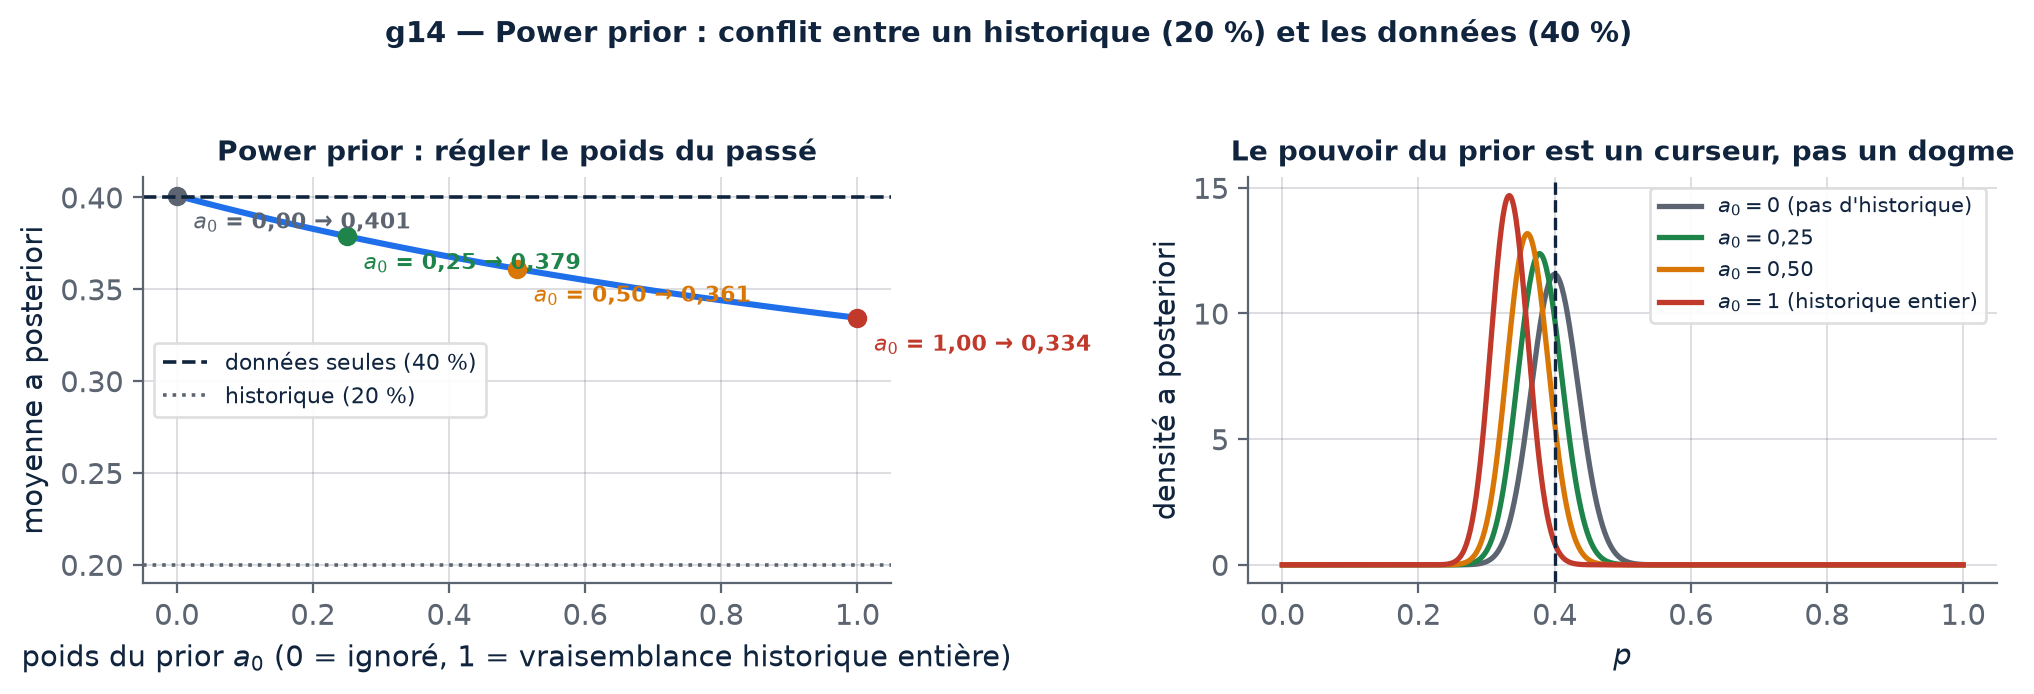
\includegraphics[width=.88\textwidth]{g14_power_prior.png}
\end{center}
\end{frame}

\begin{frame}{Power prior : régler le poids du passé --- le curseur $a_0$}
\begin{columns}[t]
\begin{column}{0.48\textwidth}
\begin{ebox}[La situation classique de conflit]
\begin{itemize}
  \item \textbf{Historique} : $20$ succès sur $100$ essais $(p_0 = 0{,}20)$ ;
  \item \textbf{Étude actuelle} : $80$ succès sur $200$ essais $(p_1 = 0{,}40)$.
\end{itemize}
Le passé contredit le présent : un prior informatif « normal » imposerait
$0{,}20$ à des données qui disent $0{,}40$.
\end{ebox}
\end{column}
\begin{column}{0.48\textwidth}
\begin{solbox}[Le curseur $a_0$ (calculs exécutés)]
$p(\theta) \propto p(\theta \given \data_0)^{a_0}$ donne
\[
\begin{aligned}
\mathrm{Beta}\bigl(&a_0 s_0 + s_1 + 1,\\
&a_0 (n_0 - s_0) + (n_1 - s_1) + 1\bigr)
\end{aligned}
\]
\begin{center}
\resizebox{\ifdim\width>\linewidth\linewidth\else\width\fi}{!}{%
\begin{tabular}{@{}lcc@{}}
\toprule
$a_0$ & \textbf{moyenne post.} & \textbf{IC 95 \%} \\
\midrule
0 (ignoré) & 0,4010 & $[0{,}3346;0{,}4693]$ \\
0,25 & 0,3789 & --- \\
0,50 & 0,3611 & --- \\
1 (entier) & 0,3344 & $[0{,}2824;0{,}3886]$ \\
\bottomrule
\end{tabular}}
\end{center}
\end{solbox}
\end{column}
\end{columns}
\vspace{1mm}
\centering\small
\textbf{Morale} — le désaccord entre passé et présent se transforme en
\emph{paramètre} $a_0$ : le rapport d'analyse peut alors discuter, chiffre en main,
du poids à donner à l'historique.
\end{frame}

% ---------------------------------------------------------------- 5
\begin{frame}[fragile]{Prior hiérarchique : le pooling partiel}
% [rogna]
\footnotesize
\begin{columns}[t]
\begin{column}{0.54\textwidth}
\begin{codebox}[src/fig\_ch2b\_pymc.py — modèle hiérarchique non centré]
\begin{lstlisting}
se = np.array([14.9, 10.2, 16.3, 11.0,
               9.4, 11.4, 10.4, 17.6])   # erreurs types

with pm.Model() as m_h:
    mu  = pm.Normal("mu", 0, 25)          # moyenne pop.
    tau = pm.HalfNormal("tau", 10)        # dispersion inter-groupes
    z   = pm.Normal("z", 0, 1, shape=8)   # N(0,1) "centree"
    theta = pm.Deterministic("theta", mu + tau * z)
    pm.Normal("y", mu=theta, sigma=se, observed=y)

    idata = pm.sample(draws=2000, tune=1500,
                      chains=2, cores=1,
                      target_accept=0.9)
\end{lstlisting}
\end{codebox}
\end{column}
\begin{column}{0.43\textwidth}
\begin{kbox}[Théorie : trois régimes]
\[
\theta_j \sim \N(\mu, \tau^2), \qquad y_j \sim \N(\theta_j, se_j^2)
\]
\begin{itemize}
  \item $\tau \to \infty$ : \textbf{pas de pooling} — chaque groupe estimé seul ;
  \item $\tau \to 0$ : \textbf{pooling total} — un seul effet pour tous ;
  \item $\tau$ estimé : \textbf{pooling partiel} — c'est le modèle hiérarchique.
\end{itemize}
\end{kbox}
\begin{wbox}[Pourquoi la forme « non centrée »]
Écrire $\theta_j = \mu + \tau z_j$ avec $z_j \sim \N(0,1)$ évite le \emph{funnel}
(entonnoir $\mu$--$\tau$--$\theta$) qui fait diverger NUTS quand $\tau$ est petit :
même modèle, géométrie numérique différente.
\end{wbox}
\end{column}
\end{columns}
\end{frame}

% ---------------------------------------------------------------- 6
% [rogna]
% [rogna]
% [rogna]
% [split]
\begin{frame}{Shrinkage : les huit écoles se rapprochent de la moyenne}
\begin{center}
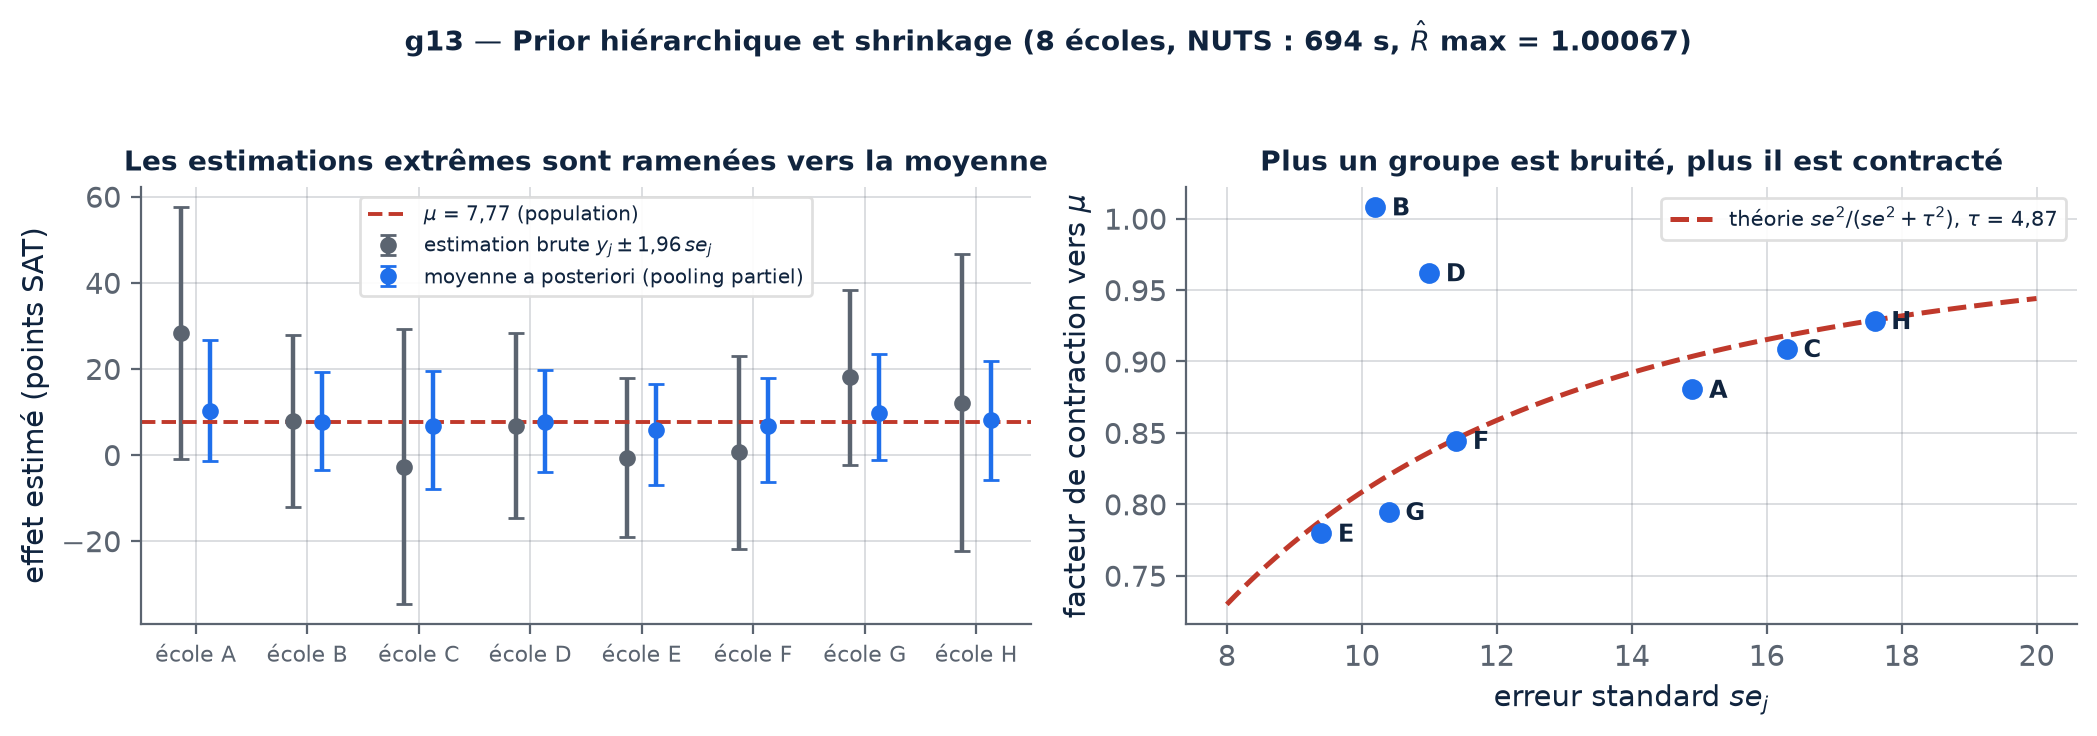
\includegraphics[width=.86\textwidth]{g13_shrinkage_8groupes.png}
\end{center}
\end{frame}

% [split]
\begin{frame}{Shrinkage : les huit écoles se rapprochent de la moyenne}

\vspace{-1mm}
\begin{columns}[t]
\begin{column}{0.55\textwidth}
\begin{ebox}[Résultats NUTS sur CPU]
$\mu = 7{,}766$, IC 95 \% $[-1{,}230 \,;\, 16{,}576]$ \;;\;
$\tau = 4{,}867$, IC 95 \% $[0{,}193 \,;\, 13{,}970]$ \; ;\;
$\hat R < 1{,}001$, ESS $> 2\,143$.
\end{ebox}
\begin{tabular}{@{}lcccccc@{}}
\toprule
\textbf{École} & A & B & C & D & E & G \\
\midrule
brut $y_j$ & 28,39 & 7,94 & $-2{,}75$ & 6,82 & $-0{,}64$ & 18,01 \\
posterior & 10,23 & 7,77 & 6,81 & 7,73 & 5,91 & 9,87 \\
contraction & 0,880 & 1,008 & 0,909 & 0,962 & 0,780 & 0,795 \\
\bottomrule
\end{tabular}
\end{column}
\begin{column}{0.42\textwidth}
\begin{kbox}[Le mécanisme, chiffré]
Largeur moyenne d'un intervalle : \textbf{49,59} points avec les données seules,
\textbf{25,27} avec le modèle hiérarchique, soit $-49$ \%. École H
($se = 17{,}6$) : contraction $0{,}929 = se^2/(se^2+\tau^2)$, exactement la
valeur théorique.
\end{kbox}
\begin{wbox}[Le piège du ratio par groupe]
Pour l'école B, dont l'estimation brute est \emph{déjà} proche de $\mu$, le ratio
observé vaut $1{,}008$ (supérieur à 1) : le ratio par groupe est instable quand
$y_j \approx \mu$. \textbf{Comparer les largeurs d'intervalles}, pas les ratios.
\end{wbox}
\end{column}
\end{columns}
\end{frame}

% ---------------------------------------------------------------- 7
\begin{frame}{Pourquoi le shrinkage est une bonne nouvelle}
% [rogna]
\small
\begin{columns}[t]
\begin{column}{0.49\textwidth}
\begin{kbox}[Compromis biais-variance]
Contracter une estimation vers une moyenne commune \textbf{introduit un biais}
(la vraie valeur d'un groupe n'est pas $\mu$) mais \textbf{réduit fortement la
variance}, parce qu'un groupe à $se$ élevé fournit peu d'information.
Le posterior tranche automatiquement en fonction de $se_j$ : c'est l'estimation
\emph{optimale} au sens de l'erreur quadratique attendue, exactement comme une
régression ridge (à cette différence que le coefficient de contraction $\tau$
est \emph{estimé} au lieu d'être réglé à la main).
\end{kbox}
\begin{ebox}[Test empirique simple]
Le modèle hiérarchique prédit un nouvel essai plus précisément que les
$8$ estimations brutes : c'est le critère qui compte, non la fidélité aux données.
\end{ebox}
\vspace{-3mm}
\end{column}
\begin{column}{0.48\textwidth}
\begin{abox}[Activité -- 10 min en binôme]
\begin{enumerate}
  \item Rejouer le modèle avec $\tau$ fixé à $0{,}1$ puis à $100$ : que
        deviennent les estimations ?
  \item Comparer à un modèle \emph{non} hiérarchique ($\theta_j$ estimés
        indépendamment, prior $\N(0,100^2)$) : qui gagne en largeur d'intervalle ?
  \item Conclure : que fait réellement l'a priori hiérarchique que ne fait
        aucun prior plat ?
\end{enumerate}
\end{abox}
\begin{solbox}[La réponse en une phrase]
Le prior hiérarchique \textbf{emprunte de l'information entre groupes} : c'est le
seul dispositif qui améliore un groupe en regardant les autres, tout en laissant
$\tau$ décider de la quantité d'emprunt.
\end{solbox}
\end{column}
\end{columns}
\end{frame}

% ---------------------------------------------------------------- 8
\begin{frame}{Quiz 3 — robustesse et shrinkage}
\begin{qbox}[Question 6 -- Quantifier la sensibilité]
\textbf{1.} Un prior $p \sim \mathrm{Beta}(50,50)$ est utilisé avec $n = 3000$
observations. Le biais potentiel du prior est-il dans l'intervalle de crédibilité ?
Conclure sur la sécurité de l'analyse. \\[1mm]
\textbf{2.} Vous avez $n = 12$ par groupe et $8$ groupes. Pourquoi un modèle
hiérarchique est-il préférable à huit estimations séparées ? \\[1mm]
\textbf{3.} Un collègue propose un power prior $a_0 = 1$ avec un historique
de $10\,000$ patients. Quel est l'effet sur $w$ ? \\[1mm]
\textbf{4.} Que signifie un posterior $\tau$ dont l'IC 95 \% est
$[0{,}193 \,;\, 13{,}970]$ ? \\[1mm]
\textbf{5.} Le shrinkage peut-il créer un biais \emph{plus grand} que le biais
du prior plat ? Dans quel cas ?
\vspace{1.5mm}

\textcolor{byBlue}{\textbf{Éléments de réponse :}}
\textbf{1.} Biais $= 15/(100+3000) = 0{,}0048$ contre une sd de $0{,}0086$ :
\textbf{non}, il n'est pas visible, et c'est précisément le danger.
\quad
\textbf{2.} L'information inter-groupes remplace l'absence de données (ici
$12$ observations par groupe) ; $\tau$ est estimé, donc l'emprunt est contrôlé.
\quad
\textbf{3.} $10\,000$ patients historiques écrasent l'étude actuelle :
$w \approx 10\,000/(10\,000+n) \approx 1$ — c'est un dogme, pas un prior.
\quad
\textbf{4.} Beaucoup d'incertitude sur l'hétérogénéité : les deux extrêmes
(pooling total et absence de pooling) restent crédibles ; il faut des données
pour trancher, ou un prior faiblement informatif sur $\tau$.
\quad
\textbf{5.} Oui, si $\tau$ est forcé trop petit alors que les groupes diffèrent
réellement : on écrase une hétérogénéité réelle (sous-dispersion).
\end{qbox}
\end{frame}

% ---------------------------------------------------------------- 9
% [suite]
\begin{frame}{Pièges de la modélisation hiérarchique}
% [rogna]
\small
\begin{columns}[t]
\begin{column}{0.49\textwidth}
\begin{wbox}[Quatre façons de se tromper]
\begin{itemize}
  \item \textbf{Trop peu de groupes} : $8$ groupes suffisent à peine à estimer
        $\tau$ ; avec $3$ ou $4$, le prior sur $\tau$ pèse autant que les données.
  \item \textbf{Prior uniforme sur $\tau$} : favorise mécaniquement les grandes
        valeurs, donc l'absence de pooling (même erreur qu'en section 2.2 sur
        $\sigma$).
  \item \textbf{Funnel} : $\theta_j \sim \N(\mu, \tau^2)$ écrit directement
        ralentit ou casse l'échantillonneur quand $\tau$ est petit.
  \item \textbf{Interprétation} : $\mu$ n'est pas « l'effet moyen des 8 écoles
        \emph{observées} », c'est la moyenne de la \emph{population} dont elles
        sont un échantillon.
\end{itemize}
\end{wbox}
\end{column}
\begin{column}{0.48\textwidth}
\begin{ebox}[Les diagnostics qui le détectent]
\begin{itemize}
  \item $\hat R > 1{,}01$ ou ESS faible sur $\tau$ : suspecter le funnel ;
  \item comparer la sd estimée de $\{\theta_j\}$ à $\tau$ (elles doivent être
        compatibles) ;
  \item tracer le posterior à priori \emph{et} a posteriori sur $\tau$ : si le
        posterior reste collé au prior, les données ne disent rien — le signaler.
\end{itemize}
Nos valeurs de contrôle sur les 8 écoles : $\hat R = 1{,}00067$ pour $\mu$,
$1{,}00039$ pour $\tau$, ESS minimal $2\,143{,}6$ : les diagnostics passent.
\end{ebox}
\end{column}
\end{columns}
\end{frame}

% [suite]
\begin{frame}{Pièges de la modélisation hiérarchique (suite)}
\begin{kbox}[Et le lien avec la section 2.3 ?]
Le contrôle prédictif a priori sur $\tau$ est le seul moyen de voir qu'un
$\mathrm{HalfNormal}(10)$ prédit déjà $90$ \% des dispersions dans une plage
étroite.
\end{kbox}

\end{frame}

% ---------------------------------------------------------------- 10
\begin{frame}{Synthèse 2.4 — robustesse, sensibilité, shrinkage}
\begin{kbox}[Les cinq résultats de la section]
\begin{enumerate}
  \item Le prior domine à $n$ petit : sur $p = 0{,}35$, Beta$(50,50)$ donne
        $0{,}4909$ à $n = 10$ (décalage $+0{,}14$).
  \item Les données reprennent la main en $1/\sqrt{n}$ pour la précision
        ($0{,}1508 \to 0{,}0087$ de $n = 10$ à $3\,000$), mais le décalage du
        prior ne décroît qu'en $1/n$.
  \item Conséquence : à $n = 3\,000$, le biais résiduel ($0{,}0048$) est du même
        ordre que la sd du posterior ($0{,}0086$) — donc \textbf{dangereux}.
  \item Le power prior transforme le conflit passé/présent en curseur :
        $a_0 = 0 \to 0{,}4010$ ; $a_0 = 1 \to 0{,}3344$.
  \item Le prior hiérarchique contracte les groupes de $51$ \% en largeur
        ($49{,}59 \to 25{,}27$) avec $\tau$ estimé à $4{,}867$.
\end{enumerate}
\end{kbox}
\vspace{1mm}
\begin{ebox}[Le rapport d'analyse attendu]
Un tableau de sensibilité (au moins deux priors), les observations virtuelles de
chaque prior, la valeur de $\tau$ et l'écart de conclusion entre scénarios :
sans ces quatre éléments, l'analyse n'est pas vérifiable.
\end{ebox}
\end{frame}

% ---------------------------------------------------------------- 11
\begin{frame}{2.5 — Les recommandations de Gelman (et leur pourquoi)}
% [rogna]
\small
\begin{kbox}[Huit règles de pratique]
\begin{enumerate}
  \item \textbf{Standardiser} les prédicteurs (centrer-réduire) : un prior par
        défaut n'a de sens que sur une échelle connue.
  \item Se souvenir que \emph{le prior ne peut être compris qu'en présence de la
        vraisemblance} : $\N(0,1)$ sur un effet est très différent selon que
        $\sigma$ vaut $0{,}5$ ou $20$.
  \item Préférer un a priori \textbf{faiblement informatif} : il borne l'échelle
        sans affirmer de valeur centrale.
  \item Sur les paramètres d'échelle, utiliser des lois qui \textbf{s'éteignent}
        (demi-normale, demi-Cauchy) : jamais d'uniforme sur $\sigma$.
  \item Éviter l'uniforme sur un domaine non borné : non invariant (section 2.2).
  \item \textbf{Vérifier par un contrôle prédictif a priori} : c'est l'étape la
        plus souvent sautée, donc la plus utile.
  \item \textbf{Quantifier la sensibilité} au lieu de la craindre : deux priors,
        deux conclusions, on dit l'écart.
  \item Réserver les priors \textbf{informatifs} aux cas où l'information existe :
        réplication, essai antérieur.
\end{enumerate}
\end{kbox}
\vspace{1mm}
\centering\small
Chaque règle s'accompagne d'un diagnostic qui la rend vérifiable — c'est ce que
fait ce chapitre.
\end{frame}

% ---------------------------------------------------------------- 12
\begin{frame}{Standardisation : la règle qui simplifie tout}
% [rogna]
\footnotesize
\begin{columns}[t]
\begin{column}{0.52\textwidth}
\begin{ebox}[Mise en oeuvre]
\[
z = \frac{y - \bar y}{s_y}, \qquad
\text{puis } z \sim \N(0, 1) \text{ a priori}
\]
Sur les 8 écoles (effets en points SAT) : moyenne $8{,}820$, écart-type
$10{,}514$. Après standardisation, les effets deviennent
$\mathbf{1{,}861}$, $\mathbf{-0{,}084}$, $\mathbf{-1{,}100}$, $\mathbf{-0{,}190}$,
$\mathbf{-0{,}900}$, $\mathbf{-0{,}779}$, $\mathbf{0{,}874}$, $\mathbf{0{,}318}$.
Le même prior $\N(0,1)$ est alors recommandé pour toutes les études.
\end{ebox}
\end{column}
\begin{column}{0.45\textwidth}
\begin{kbox}[Trois bénéfices immédiats]
\begin{itemize}
  \item Le prior devient \textbf{transposable} d'une étude à l'autre ;
  \item la \emph{condition} numérique du modèle s'améliore (MCMC plus rapide,
        section 2.4 : $693{,}7$~s pour $8$ groupes non standardisés) ;
  \item l'a priori faiblement informatif n'est plus une boîte noire :
        $\N(0,1)$ sur $z$ dit « un effet d'un écart-type du phénomène, pas plus ».
\end{itemize}
\end{kbox}
\begin{wbox}[L'erreur classique en régression]
Mettre $\N(0, 100^2)$ sur des coefficients non standardisés : le prior couvre
$100$ unités d'un prédicteur en euros, mais aussi bien $100$ unités d'un
prédicteur en milliards. La standardisation rend le prior comparable — et le
contrôle prédictif a priori le prouve.
\end{wbox}
\end{column}
\end{columns}
\end{frame}

% ---------------------------------------------------------------- 13
\begin{frame}{Les pièges classiques — et leur remède}
\centering
\renewcommand{\arraystretch}{1.15}
\small
\begin{tabular}{@{}p{7.4cm}p{4.6cm}@{}}
\toprule
\textbf{Piège} & \textbf{Remède} \\
\midrule
« non informatif » sur un taux : Beta$(0{,}5;0{,}5)$ donne
$P(p<0{,}1) = 0{,}2048$ & comparer à Beta$(1,1)$, contrôler le prédictif \\[1mm]
uniforme sur un écart-type : $P(\sigma > 50) = 0{,}5$ et
$P(|y| > 100) = 0{,}094$ & demi-normale ou uniforme sur $\log\sigma$ \\[1mm]
prior trop fort : Beta$(50,50)$, soit $w = 0{,}813$ face à 23 vols &
compter les observations virtuelles $a+b$ \\[1mm]
prior impropre : posterior parfois impropre, sortie MCMC fausse en silence &
vérifier $\int p(y \given \theta)p(\theta)\mathrm{d}\theta < \infty$ \\[1mm]
conclure sans incertitude : « l'effet est positif » & moyenne, IC 95 \%
\emph{et} $P(\theta > \text{seuil})$ \\[1mm]
\bottomrule
\end{tabular}
\vspace{-1mm}
\begin{qbox}[Question 7 -- Diagnostic express]
Un script annonce un prior Beta$(50,50)$ « non informatif » : quel chiffre
dénonce l'erreur ? \quad \textcolor{byBlue}{\textbf{Réponse :}} $w = 0{,}813$, soit
$98$ observations virtuelles.
\end{qbox}
\end{frame}

% ---------------------------------------------------------------- 14
% [suite]
\begin{frame}{Bonnes pratiques : la checklist opérationnelle}
\begin{columns}[t]
\begin{column}{0.49\textwidth}
\begin{abox}[Avant de voir les données]
\begin{enumerate}
  \item Écrire le modèle (vraisemblance, paramètres, échelles).
  \item Standardiser les variables et vérifier les unités.
  \item Choisir le prior, écrire $a+b$ / $n_0$ / $\tau$ et \emph{pourquoi}.
  \item Faire tourner le \textbf{contrôle prédictif a priori} ;
        citer un événement prédit impossible le cas échéant.
  \item Si historique : décider le power prior $a_0$ \emph{avant} l'analyse.
\end{enumerate}
\end{abox}
\end{column}
\begin{column}{0.48\textwidth}
\begin{abox}[Après l'inférence]
\begin{enumerate}
  \item Diagnostics : $\hat R < 1{,}01$, ESS suffisant, traces, énergie.
  \item Contrôle prédictif a posteriori (couverture des observations).
  \item Analyse de sensibilité : au moins deux priors, un tableau de conclusions.
  \item Comparaison à une méthode non informative du résultat (MLE, IC classique).
  \item Rapport : modèle, prior, contrôles, écarts de conclusion, limites.
\end{enumerate}
\end{abox}
\end{column}
\end{columns}
\vspace{1mm}
\end{frame}

% [suite]
\begin{frame}{Bonnes pratiques : la checklist opérationnelle (suite)}
\begin{ebox}[Ce que ces huit étapes remplacent]
Le débat d'opinion « il faut un prior subjectif / objectif » : chaque choix est
désormais un \emph{objet} écrit, contrôlé et testable. C'est la définition d'une
analyse reproductible.
\end{ebox}
\end{frame}

% ---------------------------------------------------------------- 15
\begin{frame}{Quiz 5 — révision générale du chapitre 2}
\begin{qbox}[Question 8 -- Bilan du chapitre]
\textbf{1.} Quel est le posterior conjugué pour $n = 23$, $k = 7$ et un prior
$\mathrm{Beta}(1,1)$ ? Donner la moyenne et l'écart-type. \\[1mm]
\textbf{2.} Citer deux a priori non informatifs et le reproche fait à chacun. \\[1mm]
\textbf{3.} Qu'est-ce que le nombre d'observations virtuelles d'un prior
Beta$(a,b)$ ? Quelle est sa valeur pour Beta$(1{,}3;50)$ ? \\[1mm]
\textbf{4.} Écrire la conséquence du contrôle prédictif sur
$\sigma \sim U(0,100)$ pour des données en points SAT. \\[1mm]
\textbf{5.} Biais en $1/n$ contre sd en $1/\sqrt{n}$ : lequel est le plus dangereux
à $n = 3\,000$, et pourquoi ? \\[1mm]
\textbf{6.} Que fait un prior hiérarchique qu'aucun prior plat ne peut faire ?
\vspace{1.5mm}

\textcolor{byBlue}{\textbf{Réponses :}}
\textbf{1.} Beta$(8,17)$ ; moyenne $0{,}3200$, écart-type $0{,}0915$.
\quad
\textbf{2.} Uniforme (non invariant par reparamétrisation, souvent impropre) et
Jeffreys (favorise les extrêmes, $P(p<0{,}1) = 0{,}2048$).
\quad
\textbf{3.} $a+b-2$ (ou $a+b$ selon la convention) ; $51{,}3 - 2 = 49{,}3$.
\quad
\textbf{4.} Il prédit $P(|y|>100) = 0{,}094$ : des effets absurdes pour un test
scolaire ; il faut $\log\sigma$ ou une demi-normale.
\quad
\textbf{5.} Le biais : à $n = 3\,000$ il vaut $0{,}0048$ contre une sd de
$0{,}0086$, donc il est \emph{invisible dans l'intervalle} tout en faussant le centre.
\quad
\textbf{6.} Emprunter de l'information entre groupes, avec une quantité
d'emprunt ($\tau$ estimé à $4{,}867$ ici) déterminée par les données.
\end{qbox}
\end{frame}

% ---------------------------------------------------------------- 16
\begin{frame}{Synthèse du chapitre 2 — et ce qui vient ensuite}
\begin{columns}[t]
\begin{column}{0.49\textwidth}
\begin{kbox}[Le chapitre en cinq phrases]
\begin{enumerate}
  \item Le posterior n'est pas calculé, il est \textbf{reconnu} : quatre couples
        conjugués couvrent l'essentiel des cas d'école.
  \item Un prior se \textbf{mesure} : taille d'échantillon virtuelle, invariance,
        propriété (propre ou impropre).
  \item Un prior se \textbf{teste} : contrôle prédictif a priori, avant de
        regarder les données.
  \item Un prior se \textbf{quantifie} : sensibilité en $1/n$, incertitude en
        $1/\sqrt{n}$, et c'est le biais qui survit aux grands échantillons.
  \item Un modèle hiérarchique \textbf{emprunte} de l'information entre groupes :
        $49{,}59 \to 25{,}27$ de largeur sur les 8 écoles.
\end{enumerate}
\end{kbox}
\end{column}
\begin{column}{0.48\textwidth}
\begin{ebox}[Passerelle vers le chapitre 3]
Le posterior est maintenant une \emph{loi}. Le chapitre 3 lui pose les questions de
l'inférence : comment le \textbf{résumer} (moyenne, mode, médiane) ? comment
construire un \textbf{intervalle de crédibilité} ? comment \textbf{tester une
hypothèse} par région de crédibilité ? comment \textbf{prédire} une observation ?
\end{ebox}
\begin{tcolorbox}[colback=byCyan!8,colframe=byCyan,arc=2mm]
\small\centering
\textbf{À faire avant la séance suivante} — \textbf{TP2} :
\file{notebooks/TP2\_priors\_\allowbreak conjugaison\_shrinkage.ipynb}. Y changer
le prior d'élicitation et recalculer le tableau de sensibilité.
\end{tcolorbox}
\end{column}
\end{columns}
\end{frame}
